\section{Basics of Signal Jamming}
\subsection{Introduction}

\paragraph{Jamming:} Entirely preventing or reducing the ability of communicating parties to pass information by the deliberate use of EM signals.

\paragraph{Symbols:} Can carry one or more bits of information, depending on the modulation scheme.

\paragraph{Symbol Jamming:} Corrupt symbols such that the receiver either cannot interpret them or interprets them incorrectly
\begin{itemize}
    \item Most communication systems will do error detection and
    correction
    \item Beyond a certain threshold of corrupted bits (given for each ECC scheme) the messages cannot be recovered.
    \item [$\rightarrow$] Targeted low-power jamming of individual bits is not easy and might require synchronization.
\end{itemize} 

\paragraph{Communication Jamming:} Corrupt enough bits such that the information cannot be reconstructed (despite Error Correction). 
\begin{itemize}
    \item Frequency: To jam, the attacker needs to transmit on the right
    frequencies during the right time. (e.g., all or strongest frequency). Partial jamming might not prevent communication.
    \item However, attacker can jam most dominant frequencies and these are likely most important ones for signal transmission. 
    \item Note: Receiver filters signals to the frequencies that he wishes to here, so only jamming w.r.t these frequencies will have effect. 
\end{itemize}

\begin{minipage}{\linewidth}
    \centering      
    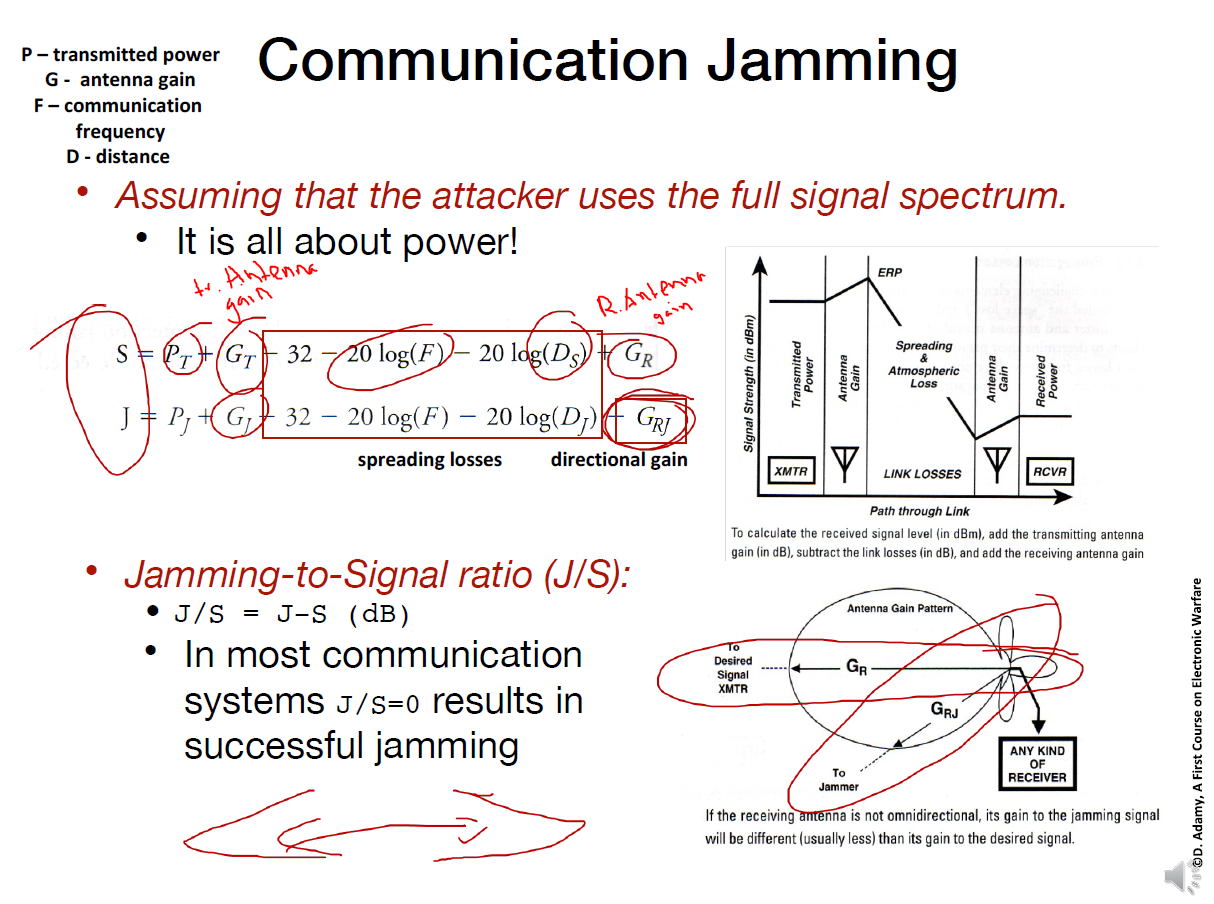
\includegraphics[width=\linewidth]{Figures/L2_communication_jamming.PNG} 
\end{minipage}

\paragraph{Burn-through range:} The range from which the sender
succeeds in communicating with the receiver, despite jamming.

\begin{minipage}{\linewidth}
    \centering      
    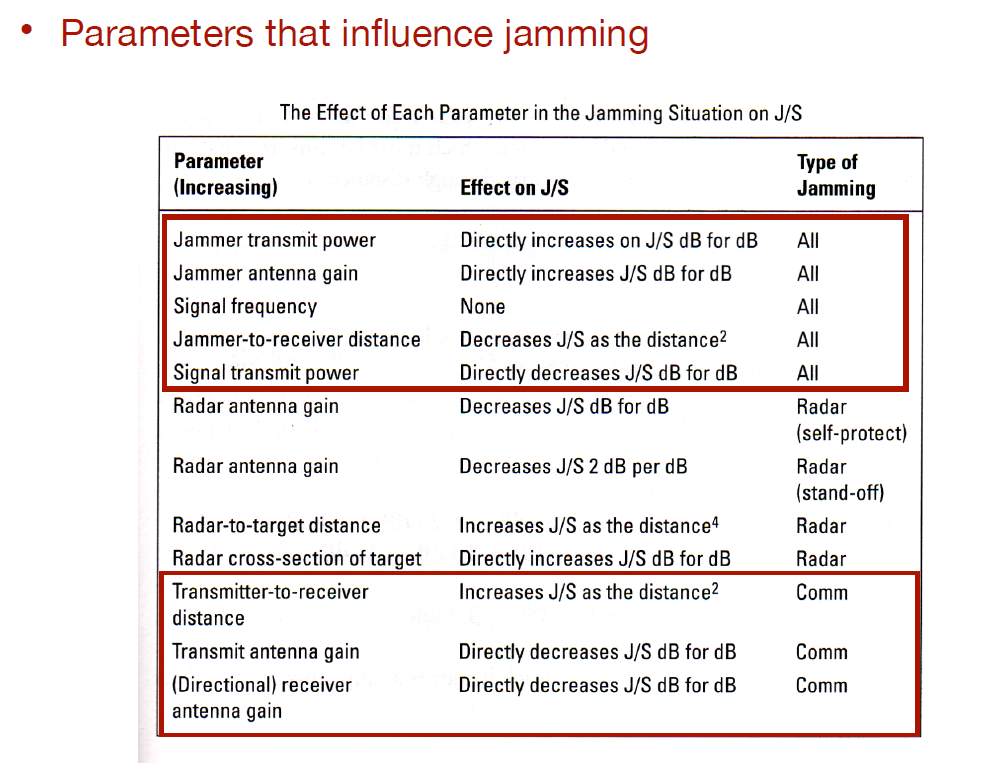
\includegraphics[width=\linewidth]{Figures/L2_jamming_params.PNG} 
\end{minipage}

\paragraph{Jamming Implications:} 
\begin{itemize}
    \item Denial of Service attacks
    \item Trick Public WiFi Localization Systems by jamming legitimate Access Points and inserting MACs of APs from other location.
    \item
\end{itemize}

\subsection{Physical Layer Security}

\paragraph{Basic Principle of Jamming Resistant Communication:} If you cannot fight, RUN, HIDE (and WAIT). But we need an advantage over the attacker: \textcolor{blue}{a shared secret key between the sender and the receiver}

\subsubsection{Frequency Hopping Spread Spectrum FHSS}
\begin{minipage}{\linewidth}
    \centering      
    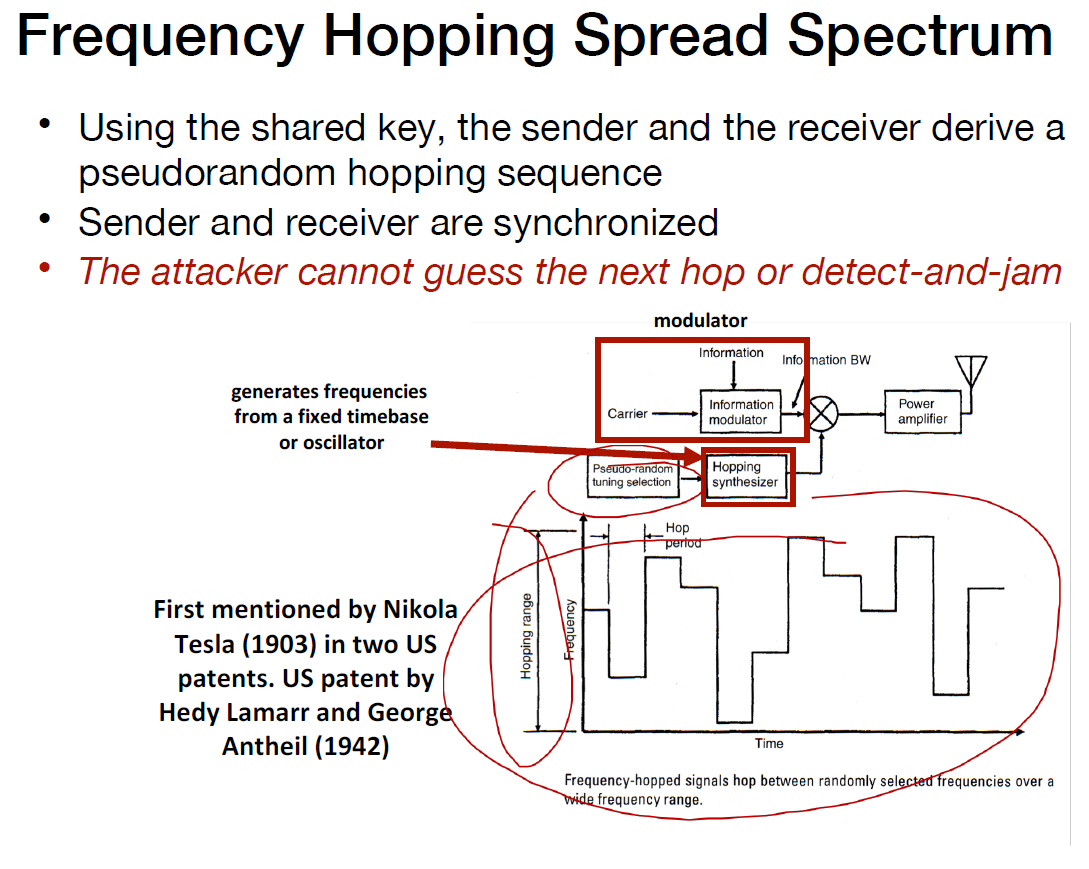
\includegraphics[width=\linewidth]{Figures/L2_frequency_hopping.PNG} 
\end{minipage}

$\rightarrow$ FHSS makes Partial Band Jammers useless.

\paragraph{Follower Jammer}
\begin{itemize}
    \item First detects on which frequency communication is taking
    place and then jams.
    \item Protection: message encodings that enable message
    recovery despite of x\% of it being corrupted
\end{itemize}

\paragraph{Detectability/Localization of FHSS transmitters}
\begin{itemize}
    \item FHSS transmitters do not really hide.
    \item Using AoA (Angle of Arrival) techniques can be localized.
\end{itemize}

\subsubsection{Direct Sequence Spread Spectrum (DSSS)}

\begin{minipage}{\linewidth}
    \centering      
    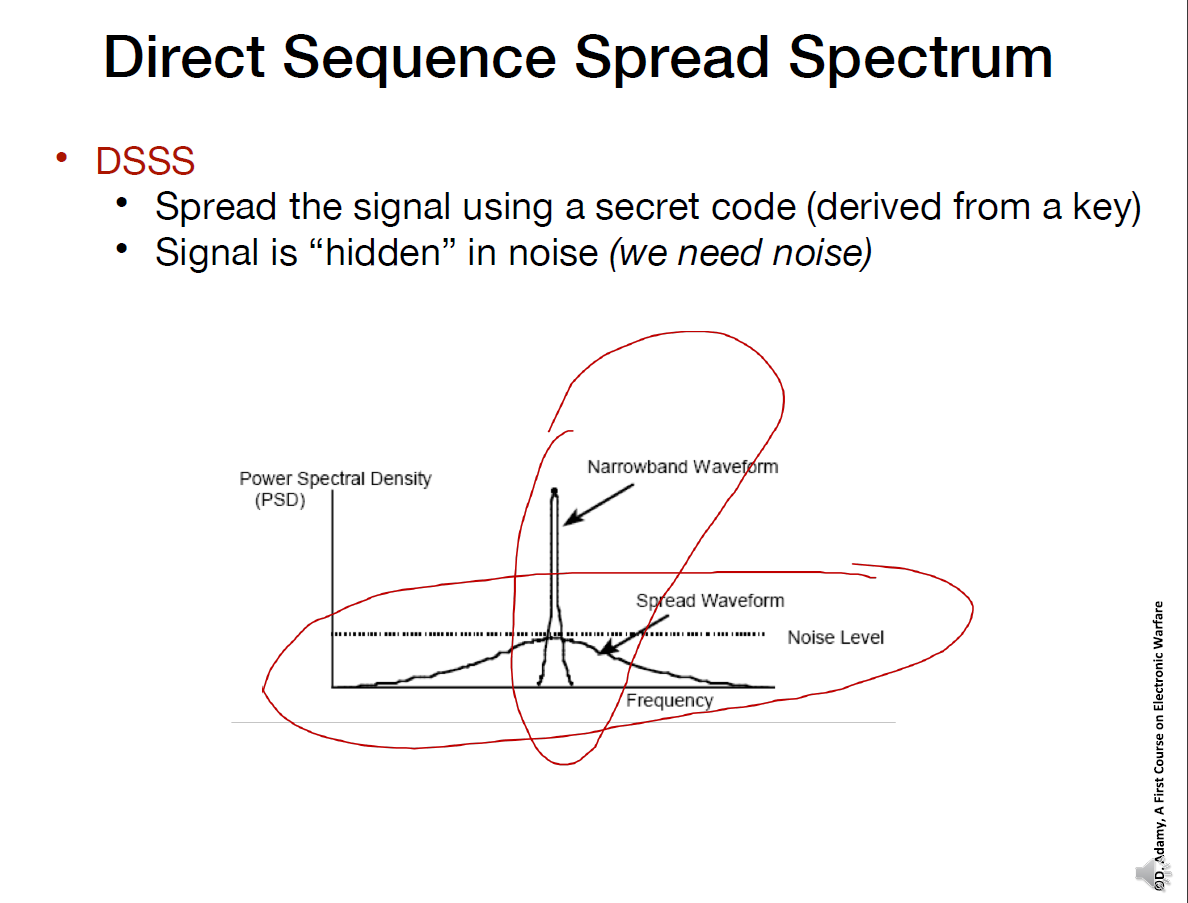
\includegraphics[width=\linewidth]{Figures/L2_DSSS.PNG} 
\end{minipage}

\paragraph{Spreading the frequency bandwidth to achieve DSSS:}
\begin{itemize}
    \item To spread, we need to transmit with a higher symbol rate.
    \item The original message is multiplied (xored) with a higher frequency spreading code (chips) that is either flipped for 0 or not for 1.
    \item This results in a signal with higher frequency bandwidth but lower signal power (per frequency band.
    \item Spreading code generator accepts a secret key.
    \item DSSS protects against Narrow-band jamming (now needs much higher power), because The same process that collapses the frequency spectrum of the spread-spectrum signal back to its information bandwidth spreads any nonsynchronized narrowband signal by the same factor
    \item Broad-band jamming is still effective (if you have enough power). Broadband jamming signal stays spreaded after passing through the spreading demodulator, unless its spreading is synchronized with the secret spreading code of the demodulator.
    \item Hides the Signal in noise! Signal Detection is more difficult. (Can be done)
    \item Processing gain = $10 log_{10}(f_{spread} / f_{unspread})$
\end{itemize}

\subsubsection{Chirp Signals} 
Random start and then sweep (can be used with FH)
\begin{itemize}
    \item Prevents narrow-band and partial-band jamming
    \item Follower jammers might be an issue
\end{itemize}

\begin{minipage}{\linewidth}
    \centering      
    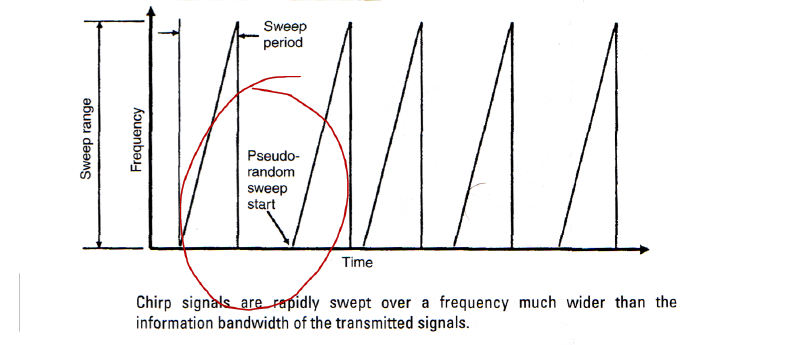
\includegraphics[width=\linewidth]{Figures/L2_chirp_signals.PNG} 
\end{minipage}

\subsection{Further Info}
\begin{itemize}
    \item Difficult to defend against can be only made more difficult.
    \item Typically combined with jammer detection and "neutralization".
    \item 802.11b uses DSSS but for interference resilience
\end{itemize}
